\documentclass[11pt]{article}
\usepackage[margin=1in]{geometry}
\usepackage{amsmath,amssymb,amsthm}
\usepackage{enumitem}
\usepackage{graphicx}
\usepackage{booktabs}
\usepackage{float,caption}
\usepackage[colorlinks=true,urlcolor=blue,linkcolor=black]{hyperref}

\newtheorem*{theorem*}{Theorem}
\newcommand{\E}{\mathbb{E}}
\newcommand{\R}{\mathbb{R}}
\newcommand{\N}{\mathbb{N}}

\title{DATA 37711: Machine Learning \& AI Part I\\Homework 3}
\author{Hetav Mehta}
\date{Fall 2026}

\begin{document}
\maketitle

\begin{center}
Code: \url{https://github.com/HetavMehta999/STAT-37711-Homework/tree/main/homework_3}
\end{center}

%======================================================================
\section*{Problem 1}

\subsection*{(a)}
\textbf{i.} $Y$ is a count, and the Poisson is a distribution on exactly $\{0,1,2,\dots\}$, the standard
model for the number of events occurring independently at some rate. It has a single parameter, the
mean $\mu=\E[Y\mid X]$, so we only need to learn one function of $X$. Its variance equals its mean,
which matches the typical behaviour of counts.

\textbf{ii.} The Poisson rate must be positive, but $f(X)=\sum_j\lambda_j h_j(X)$ can be any real number.
$\exp:\R\to(0,\infty)$ maps every $f$ to a valid rate, so boosting can add trees without constraints.
It is also the canonical link: $p(y\mid\mu)=\frac{1}{y!}\exp(y\log\mu-\mu)$ has natural parameter
$\log\mu$. This makes the loss below convex in $f$ with a simple gradient.

\subsection*{(b)}
The loss is the negative log-likelihood. Dropping $\log Y!$, which does not depend on $f$:
\[
  L\big(Y,f(x)\big) = e^{f(x)} - Y f(x), \qquad \hat R(f)=\frac1n\sum_{i=1}^n\Big(e^{f(x_i)}-y_if(x_i)\Big).
\]

\subsection*{(c)}
\[
  \frac{dL}{df(x)} = e^{f(x)} - Y .
\]

\subsection*{(d)}
Start from the best constant, $f_0=\log\bar y$. At step $j$, compute the pseudo-residuals (negative
gradients) at the training points,
\[
  r_i = -\frac{\partial L(y_i,f)}{\partial f}\Big|_{f=f_{j-1}(x_i)} = y_i - e^{f_{j-1}(x_i)},
\]
and fit $h_j$ as the regression tree minimizing $\sum_i (r_i - h(x_i))^2$. To first order,
$\hat R(f_{j-1}+\lambda h)\approx \hat R(f_{j-1})-\frac{\lambda}{n}\sum_i r_ih(x_i)$, so this picks the tree
closest to the steepest-descent direction. Choose $\lambda_j$ by line search on
$\sum_i L(y_i, f_{j-1}(x_i)+\lambda h_j(x_i))$ (usually scaled by a learning rate), then set
$f_j=f_{j-1}+\lambda_jh_j$.

%======================================================================
\section*{Problem 2}

\noindent\textbf{Setup.} We have a training set $S$ ($n$ points) and an independent test set $T$ ($l$ points),
both i.i.d.\ from the same distribution. For each of $k$ hyperparameter settings, train
$\hat h_j=\mathcal A(S;\theta_j)$. The loss takes values in $[0,B]$. Let $R$ be the true risk,
$\hat R_T$ the test-set average, and $\hat\jmath=\arg\min_j\hat R_T(\hat h_j)$.

\subsection*{(a)}
\begin{theorem*}
With probability at least $1-\delta$,
\[
  \big|\hat R_T(\hat h_{\hat\jmath}) - R(\hat h_{\hat\jmath})\big|
  \le \max_{j\le k}\big|\hat R_T(\hat h_j) - R(\hat h_j)\big|
  \le B\sqrt{\frac{\log(2k/\delta)}{2l}} ,
\]
and consequently $R(\hat h_{\hat\jmath})\le \min_j R(\hat h_j)+2B\sqrt{\log(2k/\delta)/(2l)}$.
\end{theorem*}

\begin{proof}
Condition on $S$. Then each $\hat h_j$ is a fixed function. Since $T$ is independent of $S$, the losses
$\ell(\hat h_j(X_i),Y_i)$ are i.i.d.\ in $[0,B]$ with mean $R(\hat h_j)$. Hoeffding's inequality gives
$\Pr(|\hat R_T(\hat h_j)-R(\hat h_j)|>\varepsilon\mid S)\le 2e^{-2l\varepsilon^2/B^2}$ for each $j$. A union
bound over the $k$ settings gives
$\Pr(\max_j|\hat R_T(\hat h_j)-R(\hat h_j)|>\varepsilon\mid S)\le 2k\,e^{-2l\varepsilon^2/B^2}$. This does not
depend on $S$, so it also holds unconditionally. Setting the right side to $\delta$ gives
$\varepsilon=B\sqrt{\log(2k/\delta)/(2l)}$. Because $\hat\jmath\in\{1,\dots,k\}$, its deviation is at most
the maximum. For the second claim, let $j^\star=\arg\min_jR(\hat h_j)$. Then
$R(\hat h_{\hat\jmath})\le\hat R_T(\hat h_{\hat\jmath})+\varepsilon\le\hat R_T(\hat h_{j^\star})+\varepsilon\le R(\hat h_{j^\star})+2\varepsilon$.
\end{proof}

\noindent\emph{Remarks.} The bound depends on $l$ and $\log k$ but not on $n$: $n$ only affects how good
the candidates are. The union bound is necessary because $\hat\jmath$ is chosen using $T$. For squared
error, clip predictions to the range of $Y$; for wine, $Y\in[3,9]$ gives $B=36$.

\subsection*{(b)}
The reported score $\hat R_T(\hat h_{\hat\jmath})=\min_j\hat R_T(\hat h_j)$ is the smallest of $k$ noisy
estimates, so it is biased low:
\[
\E[\min_j\hat R_T(\hat h_j)\mid S]\le\min_jR(\hat h_j)\le R(\hat h_{\hat\jmath}).
\]
When $k$ is large relative to $l$, $\log k/l$ is no longer small and the bound in (a) becomes vacuous.
The search then fits the noise in $T$. In the extreme, with $k\ge 2^l$ binary classifiers, one of
them can have zero test error while every one has true error $1/2$. The test error stops measuring
generalization, and the chosen model may itself be worse than others. The fix is a separate held-out
set that is used only once.

\subsection*{(c)}
\textbf{Setup.} We use \texttt{winequality-white.csv} (UCI Wine Quality): 4{,}898 wines, 11
features, and target \texttt{quality}. A seeded random split gives 3{,}429 train, 490 validation and 979
test examples. Both grids have more settings than there are validation points:
{\sloppy
\begin{itemize}[leftmargin=*,itemsep=1pt]
  \item \textbf{Random forest} (600 settings): \texttt{n\_estimators} $\in\{50,100,200,400\}$,
  \texttt{max\_depth} $\in\{5,10,15,20,30,\text{None}\}$, \texttt{max\_features} $\in\{0.2,0.33,0.5,0.75,1\}$,
  \texttt{min\_samples\_leaf} $\in\{1,2,4,8,16\}$.
  \item \textbf{$k$-NN} (900 settings): \texttt{n\_neighbors} $\in\{1,\dots,50\}$,
  \texttt{weights} $\in\{\text{uniform},\text{distance}\}$, Minkowski $p\in\{1,2,3\}$, and a feature scaler
  in \{standard, min--max, robust\}, fit on train only.
\end{itemize}}
Each setting is fit on train and the one with the lowest validation MSE is selected. The test MSE of every
setting is recorded for analysis only and is never used for selection.

\begin{table}[H]
\centering\small
\begin{tabular}{lrrrrr}
\toprule
Model & \# settings & Train MSE & Val MSE & Test MSE & Test $-$ Val \\
\midrule
RandomForest & 600 & 0.051 & 0.328 & 0.395 & +0.067 \\
KNN & 900 & 0.000 & 0.360 & 0.408 & +0.049 \\
Constant (train mean) & 1 & 0.772 & 0.779 & 0.829 & +0.050 \\
\bottomrule
\end{tabular}
\\[4pt]
\begin{tabular}{ll}
\toprule
Model & Selected hyperparameters \\
\midrule
RandomForest & trees=400, depth=None, max\_feat=0.2, min\_leaf=1 \\
KNN & $k$=19, weights=distance, $p$=1, scaler=robust \\
\bottomrule
\end{tabular}

\caption*{Selected model per class. ``Constant'' predicts the training mean.}
\end{table}

\noindent The random forest does best, with test MSE $0.395$ (RMSE $0.63$); $k$-NN reaches $0.408$. Both
roughly halve the constant baseline's error ($0.829$).

\begin{figure}[H]
  \centering
  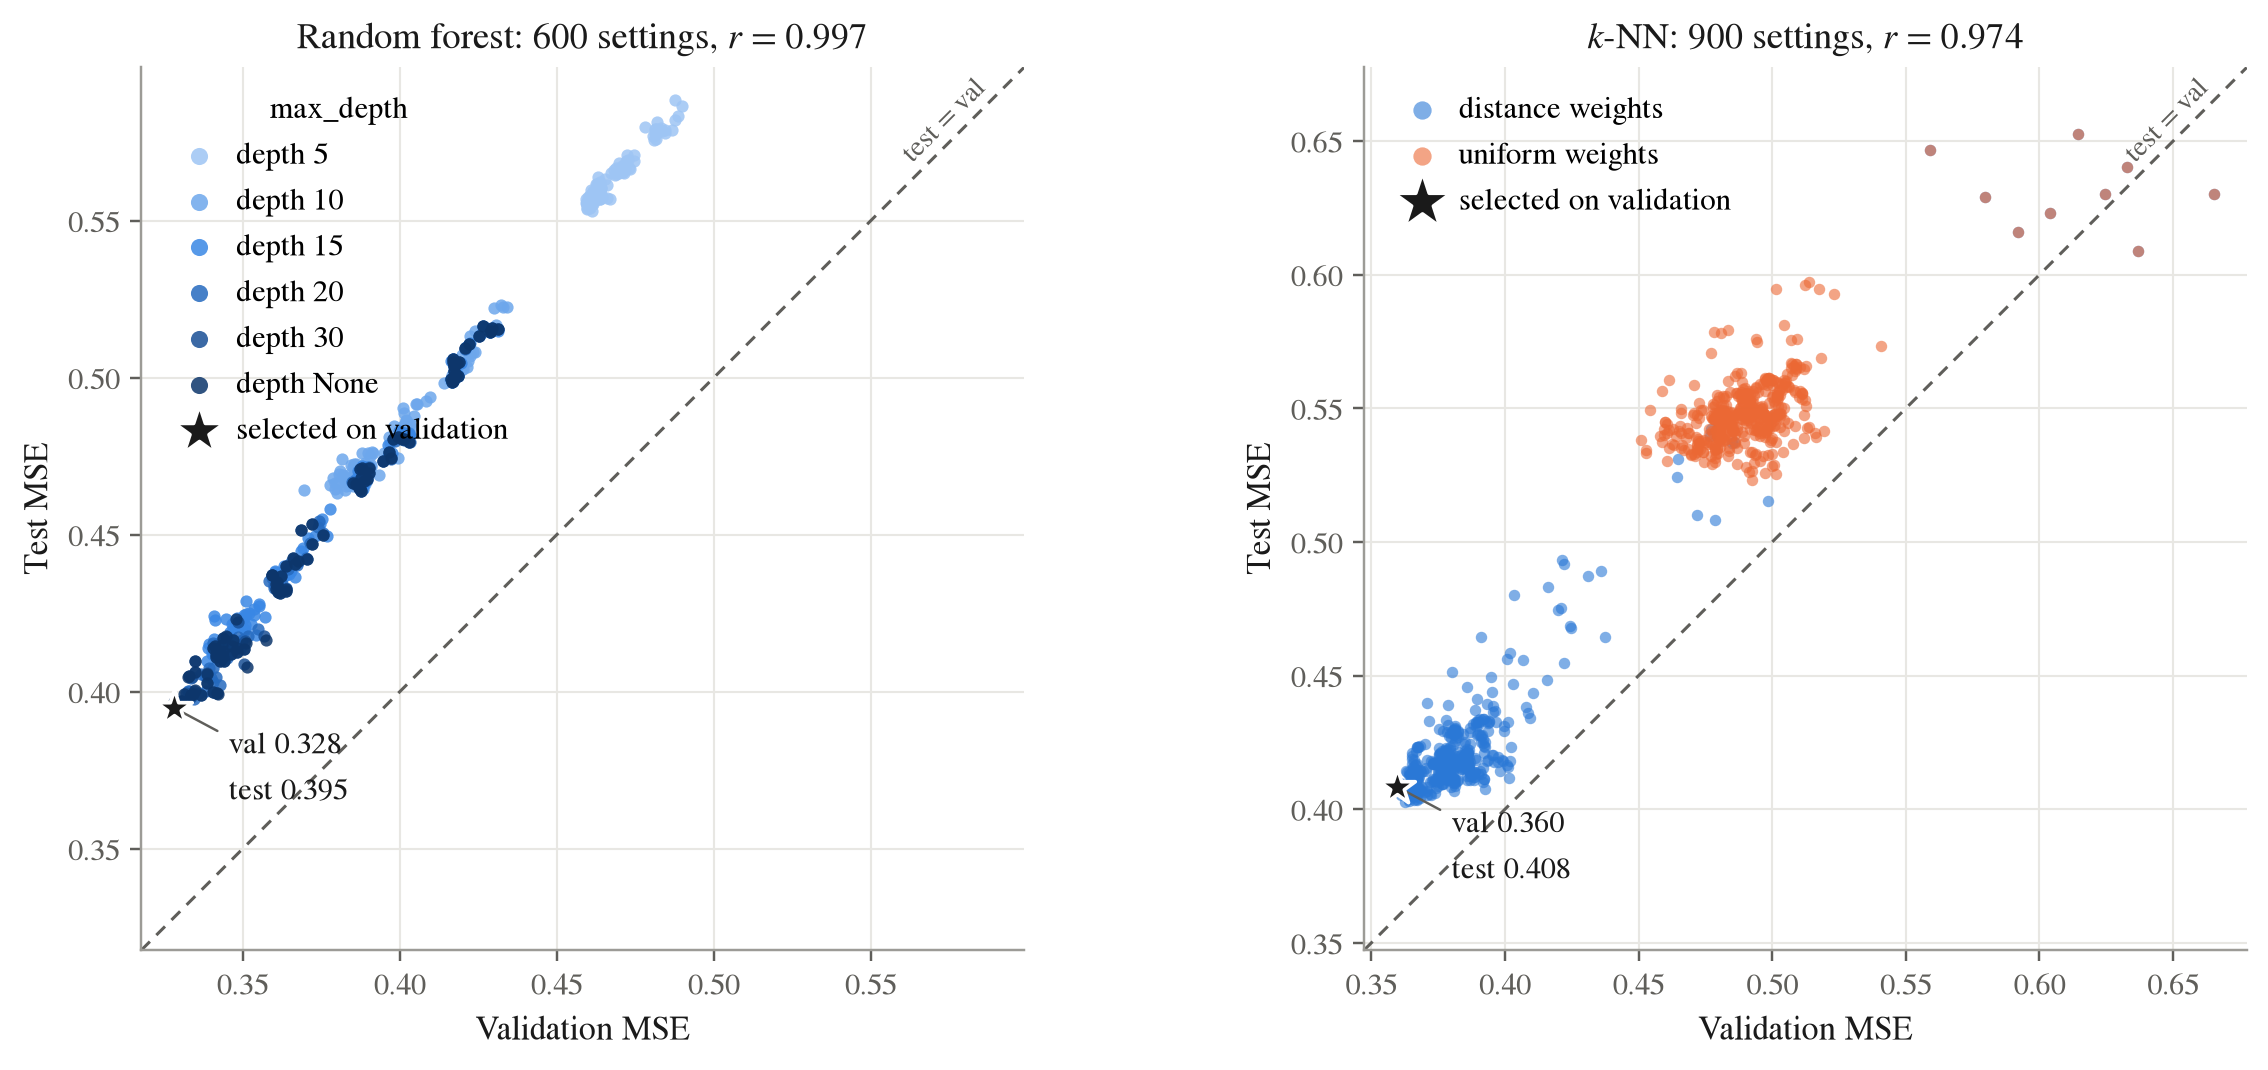
\includegraphics[width=\linewidth]{../problem2/results/val_vs_test.png}
  \caption{Validation vs.\ test MSE for every setting. The star marks the setting selected on validation.}
\end{figure}

\noindent\textbf{Validation vs.\ test risk.} The two rank settings almost identically, with correlation
$0.997$ for the forest and $0.974$ for $k$-NN. Validation therefore selects well: the forest it picks
has test MSE $0.3949$, against $0.3947$ for the best setting in hindsight. The selected model's validation
MSE is lower than its test MSE ($0.328$ vs.\ $0.395$ and $0.360$ vs.\ $0.408$), but on this split most
of that gap is split luck, since even the constant predictor has $0.779$ vs.\ $0.829$. To isolate the
selection effect, we reran the whole $k$-NN search on 30 random splits (figure below). Test exceeded
validation in 22 of 30 splits, with a mean gap of $+0.018$ (standard error $\approx0.009$). The selected
model's validation risk is an optimistically biased estimate, as (b) predicts. The test risk is
unbiased because $T$ played no part in the choice. The bias is far smaller than the bound in (a)
($\varepsilon\approx3.7$), because the settings are highly correlated and so behave like far fewer than
$k$ distinct models.

\begin{figure}[H]
  \centering
  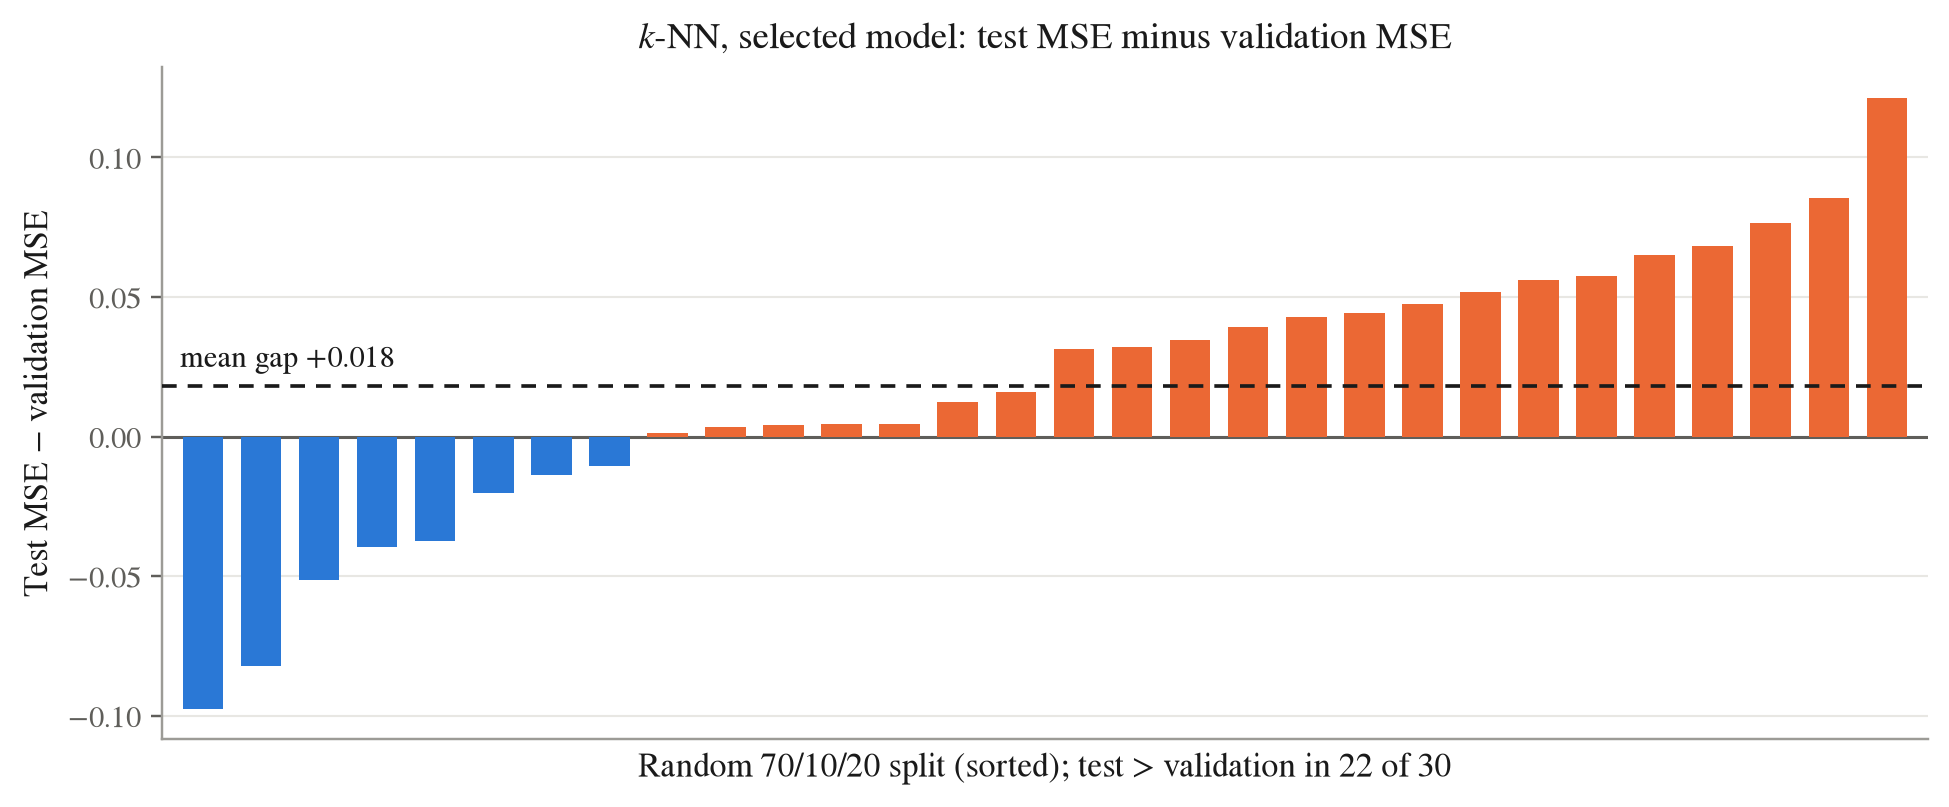
\includegraphics[width=0.85\linewidth]{../problem2/results/knn_repeated_splits.png}
  \caption{$k$-NN over 30 random splits: test MSE minus validation MSE of the selected setting.}
\end{figure}

%======================================================================
\section*{Problem 3}

\textbf{Setup.} Both datasets have 500 points, a binary label (first column) and 5 features. We fit
\texttt{GradientBoostingClassifier} (defaults: learning rate 0.1, depth-3 trees) with 1, 10, 100, 300 and
1000 trees. With only 500 points a single split is noisy, so we average over 20 random stratified 70/30
splits. The $m$-tree model equals the first $m$ stages of the 1000-tree fit; we checked this against
separate fits and they agree exactly.

\begin{table}[H]
\centering\small
\resizebox{\linewidth}{!}{\begin{tabular}{llrrrrr}
\toprule
Data & Metric & 1 tree & 10 trees & 100 trees & 300 trees & 1000 trees \\
\midrule
dset0 & Train error & 0.426 & 0.150 & 0.004 & 0.000 & 0.000 \\
 & Test error & 0.427 (0.000) & 0.275 (0.007) & 0.180 (0.006) & 0.177 (0.006) & 0.180 (0.006) \\
 & Test log-loss & 0.664 (0.001) & 0.579 (0.003) & 0.419 (0.011) & 0.480 (0.022) & 0.919 (0.056) \\
\midrule
dset1 & Train error & 0.281 & 0.114 & 0.010 & 0.000 & 0.000 \\
 & Test error & 0.319 (0.018) & 0.206 (0.006) & 0.186 (0.007) & 0.196 (0.006) & 0.200 (0.006) \\
 & Test log-loss & 0.648 (0.001) & 0.480 (0.006) & 0.409 (0.013) & 0.538 (0.022) & 1.074 (0.056) \\
\bottomrule
\end{tabular}
}
\caption*{Mean over 20 splits (standard error in parentheses).}
\end{table}

\begin{figure}[H]
  \centering
  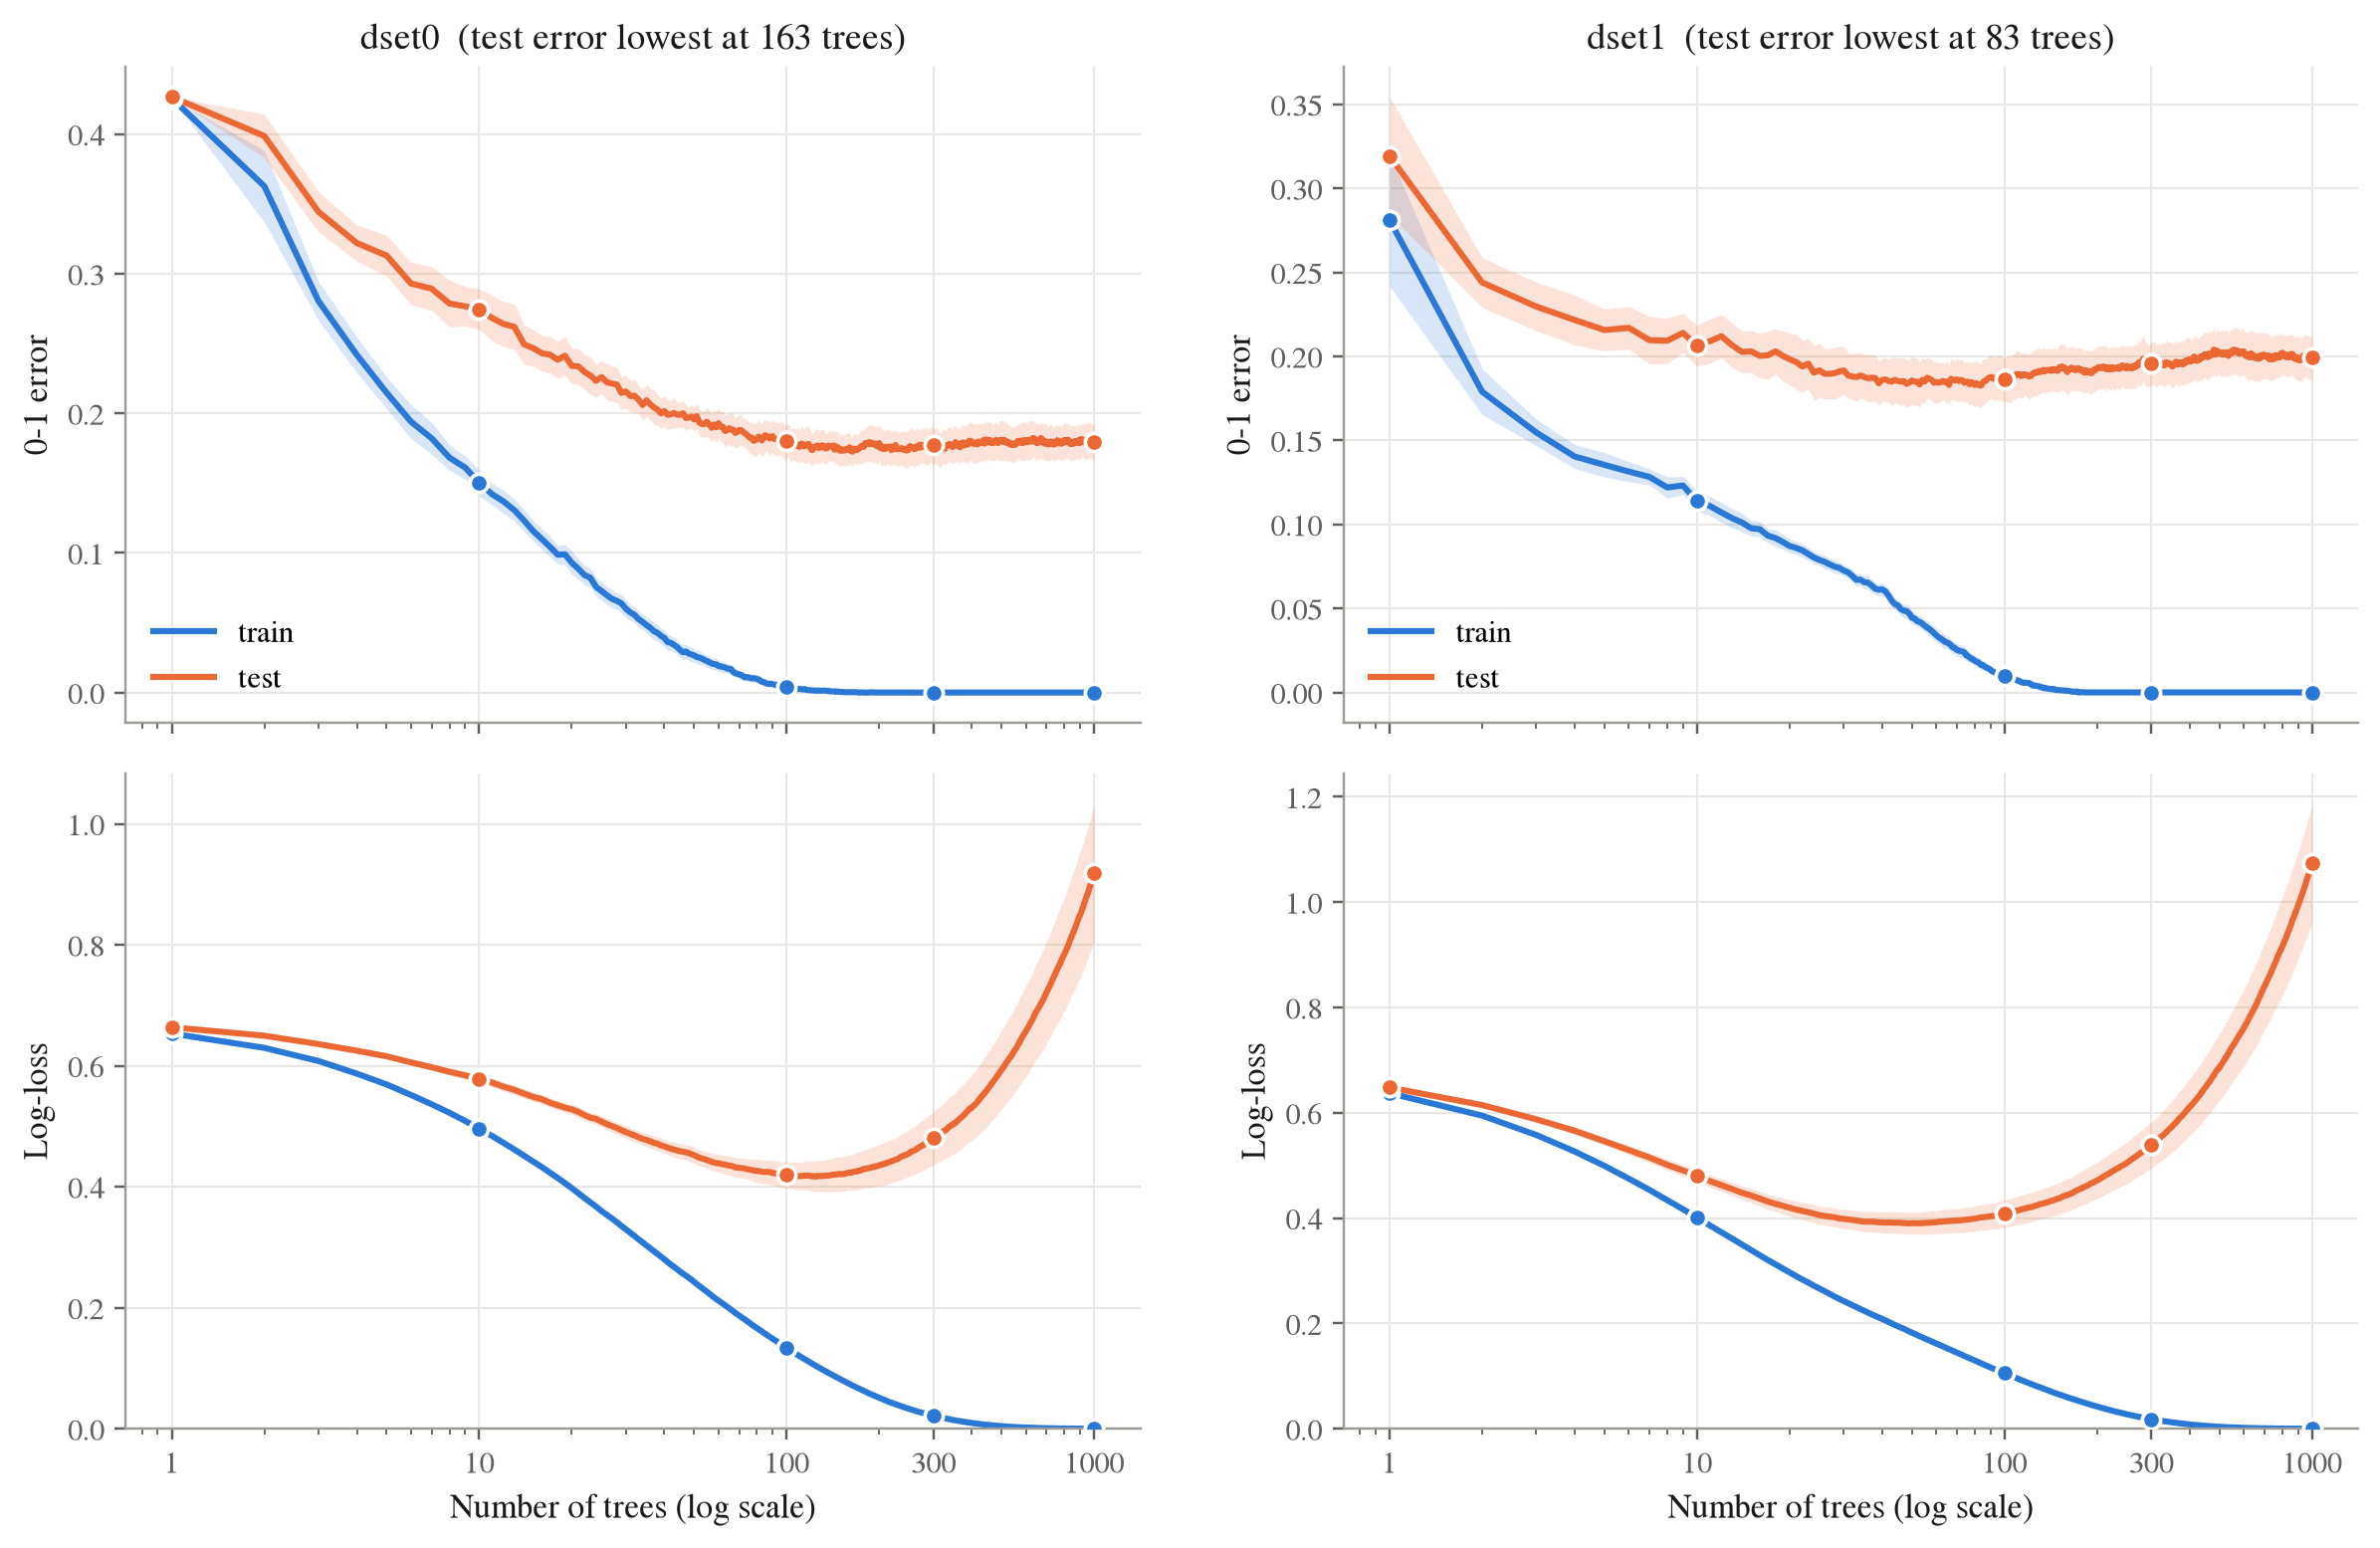
\includegraphics[width=\linewidth]{../problem3/results/error_curves.png}
  \caption{Train and test error (top) and log-loss (bottom) against the number of trees. Bands show
  $\pm2$ s.e.; dots mark 1, 10, 100, 300 and 1000 trees.}
\end{figure}

\subsection*{(a) dset0}
Training error reaches 0 by about 200 trees, yet test error does \emph{not} go back up. It falls to
about $0.18$ by 100 trees and stays there through 1000 trees. Within each split, the test error at
1000 trees minus that at 100 trees is $0.000\pm0.004$. Adding trees after the training data are fit
perfectly does not hurt test accuracy. This is the margin behaviour of boosting: later trees keep
pushing the training margins up rather than changing the decision boundary.

\subsection*{(b) dset1}
Test error is lowest at about 80--100 trees ($0.186$) and then rises steadily to $0.200$ at 1000 trees as
training error goes to 0. The paired increase from 100 to 1000 trees is $+0.013\pm0.004$, positive in
14 of the 20 splits. Here boosting does overfit, and the number of trees needs early stopping.

(On both datasets the test \emph{log-loss} rises after about 100 trees, because the model becomes
over-confident. The difference between the datasets is in classification error.)

\subsection*{(c)}
The difference is label noise. dset1 has a simple boundary with noisy labels; dset0 has a complex
boundary with little label noise.

\begin{figure}[H]
  \centering
  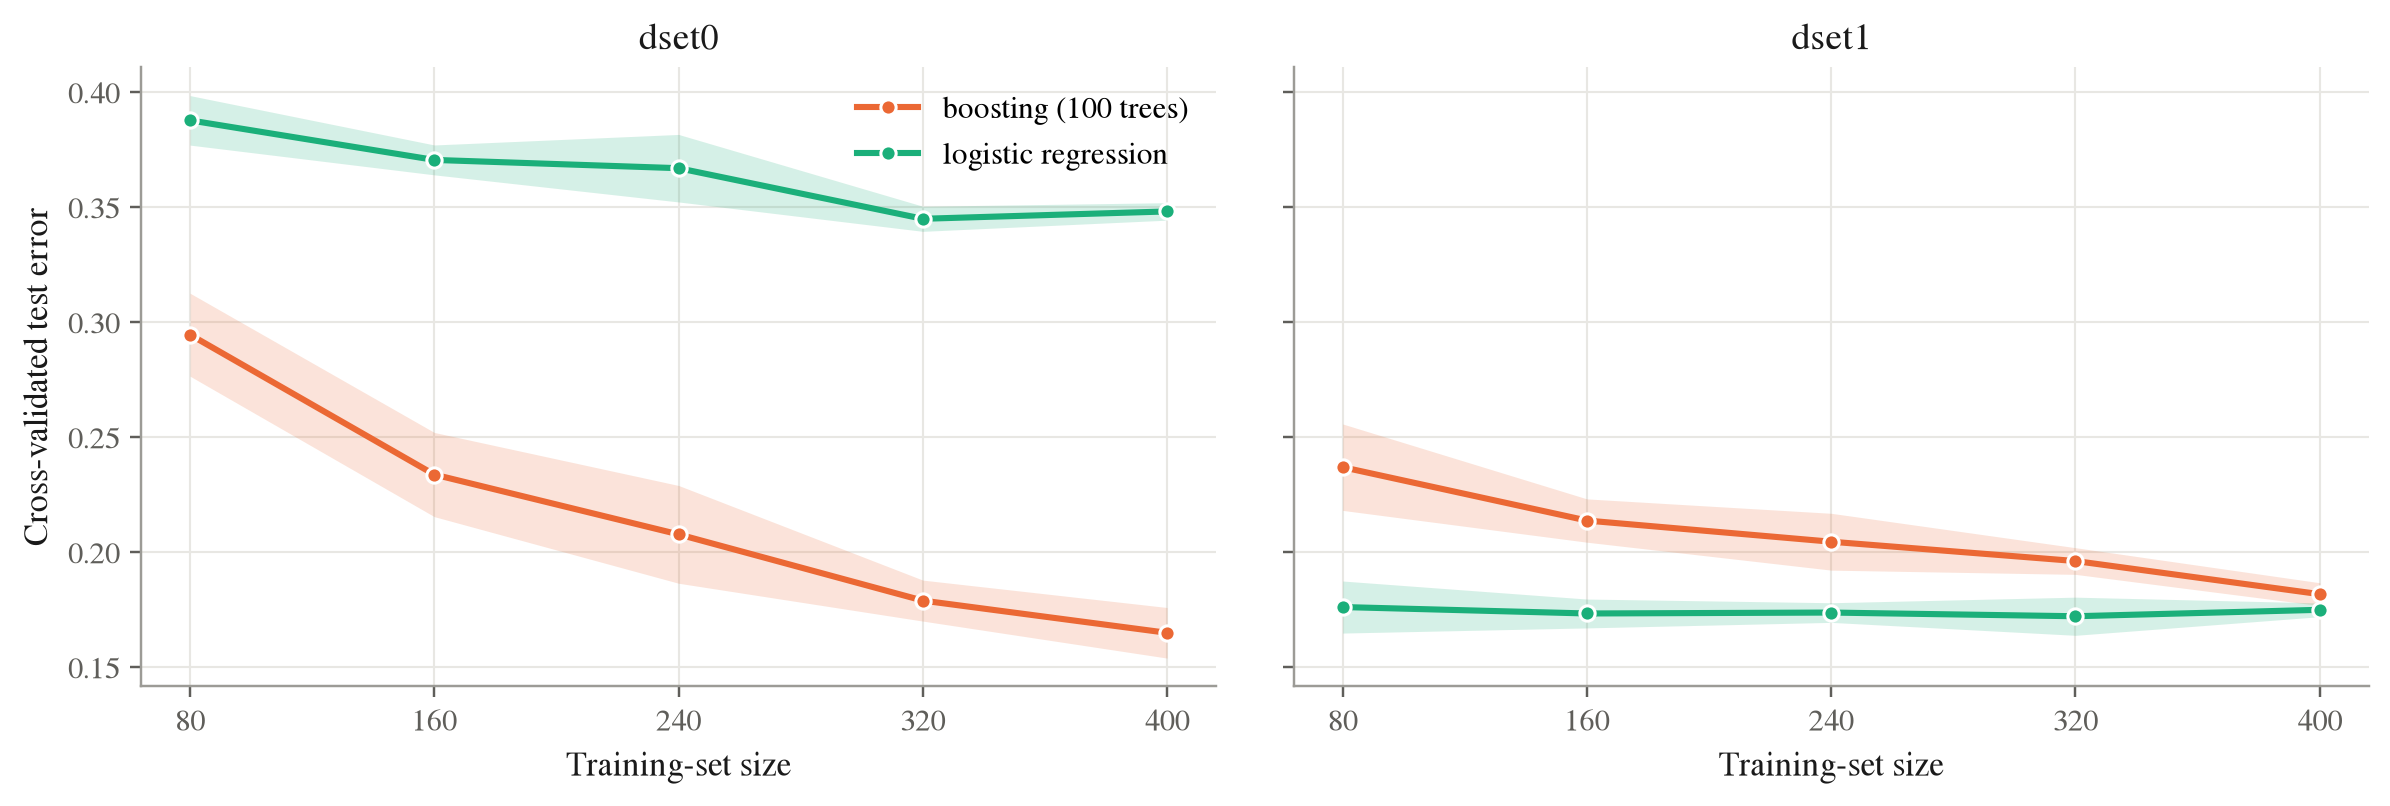
\includegraphics[width=\linewidth]{../problem3/results/learning_curves.png}
  \caption{Cross-validated test error against training-set size (5 repeats of 5-fold CV, $\pm2$ s.e.).}
\end{figure}

\noindent On dset1, plain logistic regression already reaches $0.17$ error with only 80 training points,
and does not improve with more data. Boosting never does better. So the boundary is essentially
linear, and the remaining $\approx17\%$ is irreducible: those points' labels are not determined by $X$.
Once boosting has found the boundary (about 100 trees), the only way to keep lowering training error is
to memorize these noisy labels. That carves small regions around them that misclassify nearby test
points.

On dset0, a linear model fails ($0.35$), while boosting's error keeps falling as $n$ grows. So the
remaining error comes from a complex boundary not yet learned from 350 points, not from a noise floor.
The hard training points are correctly labelled, so fitting them does not mislead the model on test
data, and test error stays flat.
\end{document}
